\chapter{Poker oraz kalkulatory szans}
\label{chapter:2}

\section{Zasady gry Poker Texas Hold’em}

Poker Texas Hold’em \cite{wiki-texas-holdem} to najpopularniejsza odmiana pokera. W standardowej rozgrywce uczestniczy od 2 graczy do 9 graczy oraz używa się pełnej talii 52 kart. Celem gry jest wygranie żetonów od innych graczy poprzez skompletowanie silniejszego układu bądź wymuszenie spasowania kart od pozostałych graczy. Każdy z graczy dysponuje dwiema kartami oraz kartami wspólnymi ujawnianymi w kolejnych rundach licytacji. Gracze w każdej turze licytacji mają do dyspozycji następujące możliwości:

\begin{itemize}
    \item Spasowanie kart (fold)
    \item Sprawdzenie (call)
    \item Podbicie stawki (raise)
    \item Czekanie (check)
\end{itemize}

Gracz może czekać tylko, gdy w obecnej turze licytacji nikt wcześniej nie podbił stawki (raise). Pojedyncze rozdanie składa się z co najwyżej 4 tur licytacji, po których dochodzi do ujawnienia kolejno: trzech kart wspólnych (flop), jednej karty wspólnej (turn) i ostatniej kart wspólnej (river). Po ostatniej turze licytacji odbywa się określenie siły rąk wszystkich graczy pozostałych w rozdaniu.

\begin{figure}[ht]
    \fbox{ \scalebox{0.74}{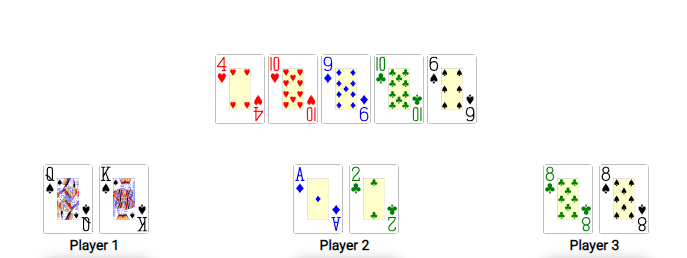
\includegraphics{images/example-hand.png}}}
    \caption{Przykładowy stan gry w trakcie ostatniej tury licytacji (river)}
    \label{fig:example-hand}
\end{figure}

Ewaluacja ręki polega na określeniu układu z poniższej listy rankingowej. Każdy z graczy do określenia swojego układu wybiera pięć kart spośród dwóch kart własnych i pięciu wspólnych.

Układy kart od najsłabszego:
\begin{description}
  \item[Wysoka karta] (High Card): Następuje w przypadku gdy układ nie kwalifikuje się pod żaden z poniższych. Gracz wybiera 5 najwyższych dostępnych dla siebie kart. Jeżeli obydwoje z graczy mają wysoką kartę należy porównać kolejno najwyższe karty. W przypadku identycznego układu następuje remis. Podobną zasadę (kicker) stosuje się w przypadku remisów w innych układach, które należy uzupełnić do 5-kartowego układu. (np. $A\clubs, T\diamonds, 7\spades, 5\hearts, 2\hearts$)
  \item[Para] (One pair): dwie karty o tej samej wartości; jeżeli gracze mają tą samą parę, decyduje kicker. (np. $A\clubs, A\diamonds, J\diamonds, 9\spades, 2\spades$)
  \item[Dwie pary] (Two pairs): Wygrywa gracz z wyższą parą; jeżeli najwyższa para jest identyczna, to wygrywa gracz z drugą najwyższą parą. Gdy druga para jest identyczna --- decyduje kicker. (np. $K\clubs, K\diamonds, T\spades, T\hearts, 4\hearts$)
  \item[Trójka] (Three of a Kind): Wygrywa gracz z trójką o wyższej randze; jeżeli ranga jest ta sama, to decyduje kicker. (np. $K\clubs, K\diamonds, K\spades, 7\hearts, 4\hearts$)
  \item[Strit] (Straight): pięć kolejnych kart; jeśli dwóch graczy ma strita to wygrywa ten, który ma wyższą kartę. W stricie as może być zarówno najwyższą jak i najniższą kartą --- jedynką. (np. $A\spades, K\diamonds, Q\clubs, J\spades, T\hearts$)
   \item[Kolor] (Flush): pięć kart w tym samym kolorze; jeśli dwóch graczy ma kolor (uzyskanie dwóch różnych kolorów jest niemożliwe) wygrywa ten, którego kolor ma najwyższą kartę. (np. $K\spades, T\spades, J\spades, 8\spades, 7\spades$)
   \item[Full] (Full house): układ składający się z trójki oraz pary; jeśli dwóch graczy ma fulla, to wygrywa ten, który ma wyższą trójkę; jeśli obydwaj mają tę samą trójkę, wygrywa ten, który ma wyższą parę; jeśli i para jest taka sama, to następuje remis. (np. $K\clubs, K\diamonds, K\spades, 4\hearts, 4\diamonds$)
  \item[Kareta] (Quads): cztery karty tej samej rangi; jeżeli obydwoje z graczy mają karetę, wygrywa ten składający się z wyższej rangi. (np. $K\clubs$, $K\diamonds$, $K\spades$, $K\hearts, 2\diamonds$)
  \item[Poker] (Straight flush): pięć kolejnych kart w tym samym kolorze; jeżeli obydwoje z graczy mają pokera, wygrywa ten z ostatnią wyższą kartą. (np. $Q\hearts, J\hearts,$ $T\hearts, 9\hearts, 8\hearts$)
\end{description}
 
\newpage{}

W scenariuszu przedstawionym na rysunku \ref{fig:example-hand} gracze dysponują następującymi układami:
\begin{itemize}
    \item Player 1: Para dziesiątek --- $T\clubs, T\hearts, K\spades, Q\spades, 9\diamonds $
    \item Player 2: Para dziesiątek --- $T\clubs, T\hearts, A\diamonds, 9\diamonds, 6\spades $
    \item Player 3: Dwie pary --- $T\clubs, T\hearts, 8\clubs, 8\spades, 9\diamonds $
\end{itemize}

Zatem gracz trzeci dysponuje najlepszym układem, drugi po nim jest gracz numer dwa, a najgorszym układem dysponuje gracz numer jeden (gracz numer dwa posiada wyższego kickera --- $A\diamonds > K\spades$).

\section{Działanie kalkulatora szans}

Zadaniem kalkulatorów szans (ang. equity calculator) jest obliczenie szansy na wygraną każdego z graczy przy wybranych przez użytkownika kartach graczy oraz kartach wspólnych --- taką sytuację dalej nazwiemy \emph{scenariuszem}. Zatem zakładamy, że każdy gracz uczestniczący w rozdaniu będzie podejmował tylko jedną akcję --- check. Wyniki z kalkulatora przydają się, do określenia rzeczywistej siły ręki przeciwko innym rękom np. przy zagraniu za wszystko (all-in) w sytuacji $Q\spades, K\spades$ vs $A\spades, A\clubs$ z kartami wspólnymi $5\diamonds, 6\hearts, Q\clubs$ gracz pierwszy ma tylko 18\% szans na wygraną.

\begin{figure}[ht]
    \fbox{ \scalebox{0.94}{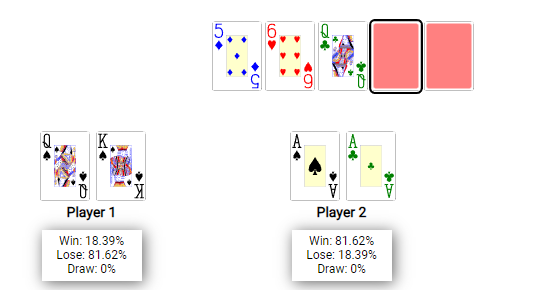
\includegraphics{images/example-hand-2.png}}}
    \caption{Wizualizacja powyższego scenariusza}
    \label{fig:example-hand-2}    
\end{figure}

Kalkulatory szans bazują na podobnej zasadzie. Należy określić, jakie karty są dostępne w talii, a następnie rozpatrzyć wszystkie możliwe kombinacje i w każdej z nich określić zwycięzcę. W scenariuszu przedstawionym na rysunku \ref{fig:example-hand-2} w talii pozostało 45 kart (52 minus po dwie karty każdego z graczy i trzy na stole). Musimy wybrać dwie z nich zatem liczba kombinacja bez powtórzeń to $\binom{45}{2}= 990$. Dla tak prostego scenariusza problem jest łatwy, natomiast w pesymistycznym i najczęstszym przypadku użycia, gdy kart w talii jest najwięcej oraz na stole nie ma żadnych kart, liczba kombinacji drastycznie rośnie, nawet do $\binom{48}{5}= 1712304$ kombinacji.

Naiwne podejście do tego problemu jest naturalne. W każdej kombinacji można posortować karty każdego z graczy, przyjrzeć się pojedynczo każdej z kart i zebrać w ten sposób potrzebne dane (np. zliczać kolory, pary) do ustalenia układu. Ten sposób ma jedną poważną wadę - jest zdecydowanie zbyt wolny do zastosowania w scenariuszach z wieloma kombinacjami. 

Wszystkie szybkie kalkulatory szans wykorzystują zapamiętane wcześniej wyniki przez naiwny algorytm lub korzystają z metody Monte Carlo \cite{monte-carlo} \cite{monte-carlo-presentation} do przybliżania wyników przy dostatecznie małym błędzie. Aplikacja  \emph{Poker Master Tool} oblicza wynik dokładnie, zatem będziemy się zajmować tylko tą metodą.

\section{Porównanie z innymi dostępnymi kalkulatorami}

\subsection{Poker Master Tool}

\href{https://pokermastertool.bartoszputek.pl/}{\emph{Poker Master Tool}} jest aplikacją internetową opartą o architekturę klient-serwer. Klient z poziomu przeglądarki w wygodny sposób wybiera interesujący go scenariusz, a następnie informacje są wysyłane do serwera, który dane przetwarza i zwraca wyświetlaną w widoku użytkownika odpowiedź. Z tego powodu do korzystania z aplikacji niezbędne jest połączenie internetowe. 

Użytkownik za pomocą myszy lub klawiatury jest w stanie wybrać karty dla każdego z graczy, karty wspólne oraz tak zwane karty martwe, wykluczone z pozostałej części talii. Informacje jakie dostajemy w zwrotnej odpowiedzi to:
\begin{itemize}
    \item Szanse na wygraną, przegraną oraz remis każdego z graczy
    \item Szanse na poszczególne układy każdego z graczy
    \item Liczbę kombinacji w danym scenariuszu
\end{itemize}

\begin{figure}[!htbp]
    \fbox{ \scalebox{0.22}{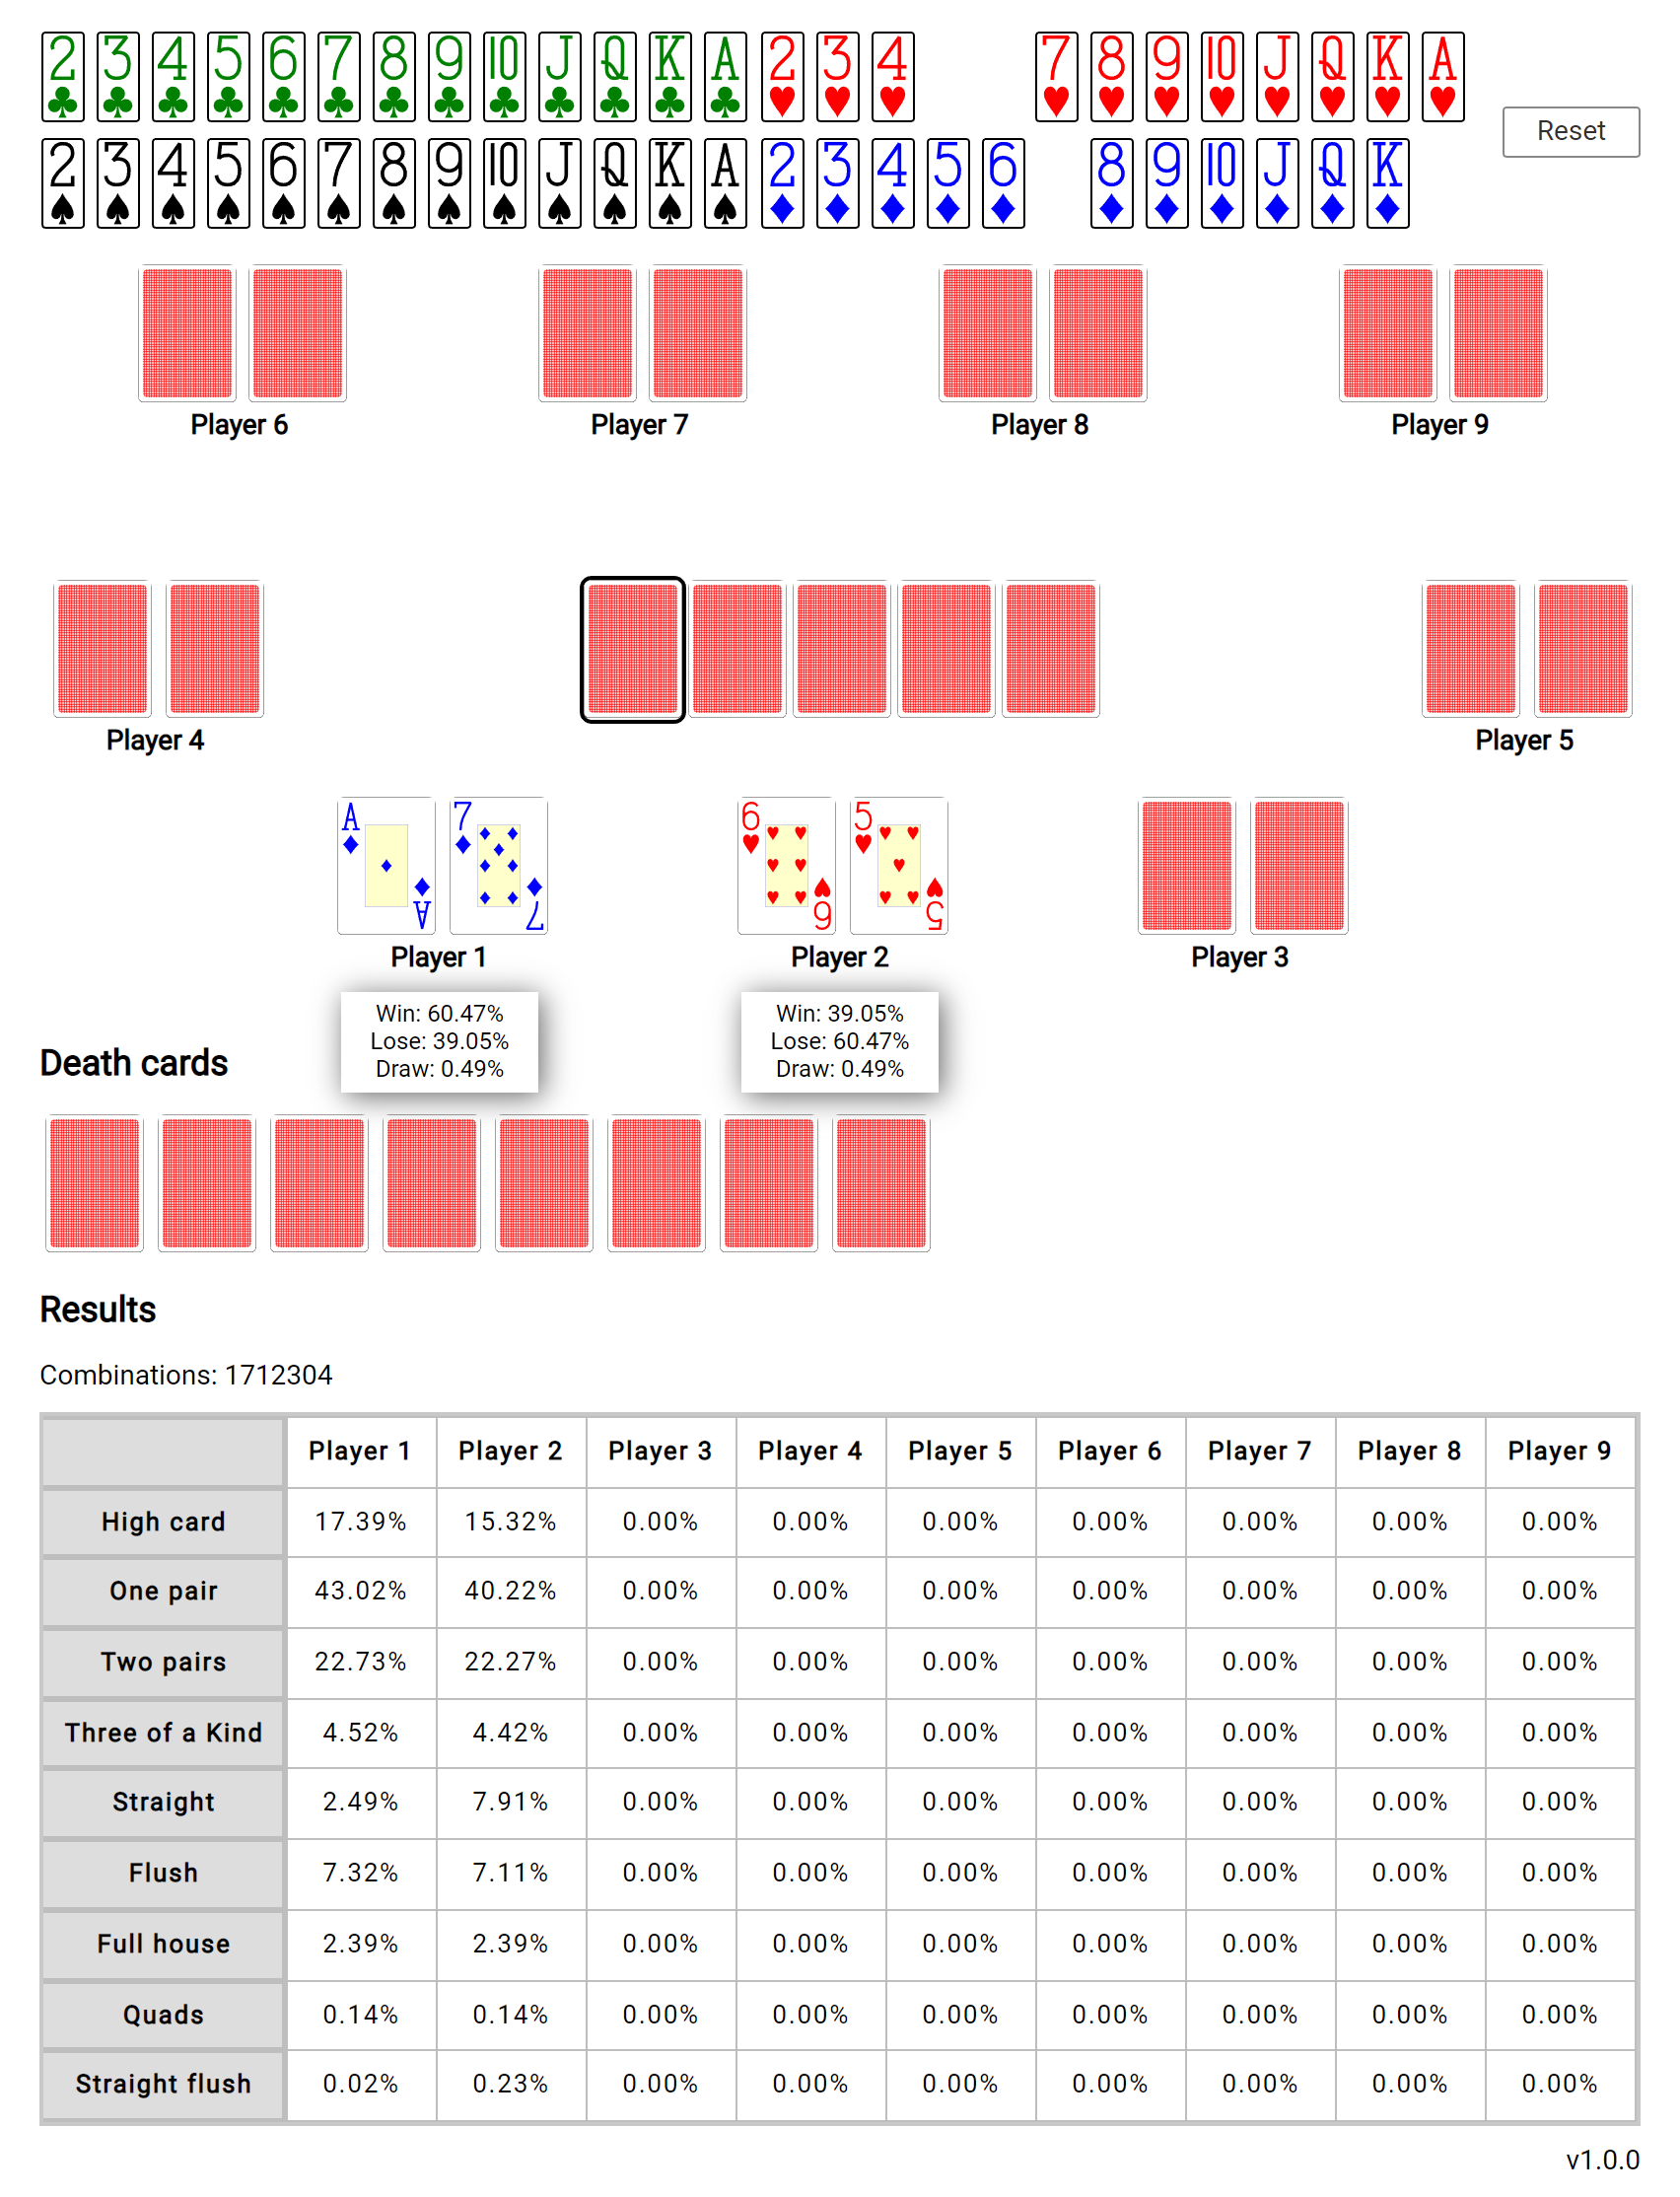
\includegraphics{images/poker-master-tool-view.png}}}
    \caption{Standardowy widok aplikacji Poker Master Tool}
    \label{fig:poker-master-tool-view}    
\end{figure}

\subsection{Power Equilab}

\href{http://power-equilab.com/}{\emph{Power Equilab}} jest płatnym oprogramowaniem przeznaczonym dla profesjonalistów w formie aplikacji desktopowej. Nie posiada wersji na telefony, za to w odróżnieniu od aplikacji webowej nie potrzebuje do działania połączenia z internetem. Jedną z jego funkcjonalności jest kalkulator szans. Kalkulator posiada wiele rozbudowanych opcji, które mogą być niejasne z perspektywy początkującego gracza, lecz bardzo przydatne dla graczy zaawansowanych. Interfejs aplikacji niestety nie pozwala komfortowo korzystać z klawiatury. 

\begin{figure}[!htbp]
    \scalebox{0.75}{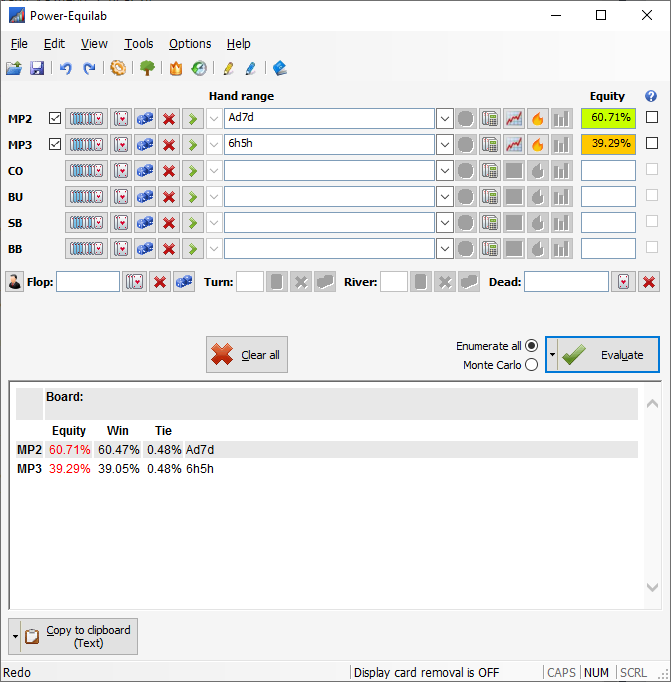
\includegraphics{images/power-equilab-view.png}}
    \caption{Standardowy widok aplikacji Power Equilab}
    \label{fig:power-equilab-view}    
\end{figure}

\subsection{Card Player Poker Odds Calculator}

\href{https://www.cardplayer.com/poker-tools/odds-calculator/texas-holdem/}{\emph{Card Player Poker Odds Calculator}} jest webowym kalkulatorem szans. Jego główną zaletą jest prostota oraz brak konieczności instalacji oprogramowania na własnym komputerze. Niestety, mimo architektury webowej trudno z niego korzystać na urządzeniach mobilnych. Nie posiada żadnych zaawansowanych funkcji oraz wynik zawiera tylko kalkulację szansy na zwycięstwo dla każdego z graczy. Interfejs nie wspiera obsługi klawiatury, a aplikacja wymaga stałego połączenia internetowego, podobnie jak w przypadku \emph{Poker Master Tool}.

\begin{figure}[!htbp]
    \scalebox{0.68}{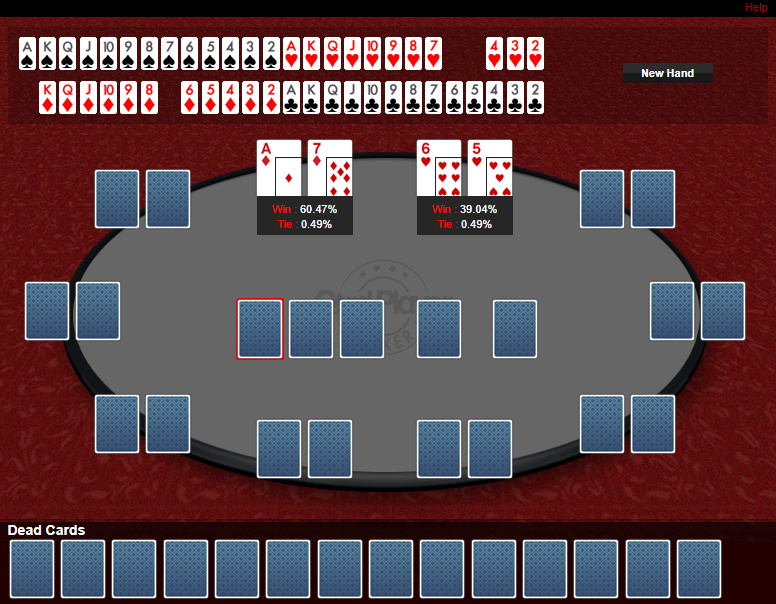
\includegraphics{images/card-player-view.png}}
    \caption{Standardowy widok aplikacji Card Player Poker Odds Calculator}
    \label{fig:card-player-view}    
\end{figure}

\begin{table}[h]
    \centering
    \begin{tabular}{lllll}
        {} & Poker Master Tool & Power Equilab & Card Player Calc.\\
        \midrule
        Typ aplikacji & Webowa  & Desktopowa & Webowa \\
        Połączenie internetowe & Tak & Nie & Tak \\
        Obsługa klawiatury & Tak & Nie & Nie \\
        Liczba funkcji & Średnia & Duża & Niska \\
        Urządzenia mobilne & Tak & Nie & Nie \\
        Przeznaczenie & Początkujący & Profesjonaliści & Początkujący \\
        Model & Darmowy & Płatny & Darmowy \\
        \bottomrule
    \end{tabular}
    \caption{Podsumowanie prezentowanych kalkulatorów}
\end{table}